\documentclass[compsoc]{IEEEtran}
\IEEEoverridecommandlockouts

\usepackage{amsmath, amssymb, amsfonts, mathrsfs}
\usepackage{balance}
\usepackage{leading}
\usepackage{graphicx}
\usepackage{subfig}
\usepackage{textcomp}
\usepackage{comment}
\usepackage{multirow}
\usepackage{framed}
\usepackage{amsmath}
\usepackage{amsthm}
\usepackage{listings}
\usepackage{xspace}
\usepackage{enumitem}
\usepackage{microtype}
\usepackage{cleveref}

 
\crefformat{section}{\S#2#1#3} 

\newcommand{\sysname}{SciSpot\xspace}




\RequirePackage[normalem]{ulem}
\RequirePackage{color}\definecolor{RED}{rgb}{1,0,0}\definecolor{BLUE}{rgb}{0,0,1}
\providecommand{\DIFadd}[1]{{\protect\color{blue}\uwave{#1}}}
\providecommand{\DIFdel}[1]{{\protect\color{red}\sout{#1}}}
\providecommand{\DIFaddbegin}{}
\providecommand{\DIFaddend}{}
\providecommand{\DIFdelbegin}{}
\providecommand{\DIFdelend}{}
\providecommand{\DIFaddFL}[1]{\DIFadd{#1}}
\providecommand{\DIFdelFL}[1]{\DIFdel{#1}}
\providecommand{\DIFaddbeginFL}{}
\providecommand{\DIFaddendFL}{}
\providecommand{\DIFdelbeginFL}{}
\providecommand{\DIFdelendFL}{}

\def\Section {\S}

\newcommand{\squishlist}{
 \begin{list}{$\bullet$}
  { \setlength{\itemsep}{0pt}
     \setlength{\parsep}{3pt}
     \setlength{\topsep}{3pt}
     \setlength{\partopsep}{0pt}
     \setlength{\leftmargin}{1.5em}
     \setlength{\labelwidth}{1em}
     \setlength{\labelsep}{0.5em} } }
	
\newcommand{\squishlisttwo}{
 \begin{list}{$\bullet$}
  { \setlength{\itemsep}{0pt}
     \setlength{\parsep}{0pt}
    \setlength{\topsep}{0pt}
    \setlength{\partopsep}{0pt}
    \setlength{\leftmargin}{2em}
    \setlength{\labelwidth}{1.5em}
    \setlength{\labelsep}{0.5em} } }

\newcommand{\squishend}{
  \end{list}  }

\newcommand{\alert}[1] {\textcolor{red} {\textsc{#1}}}

\newcommand{\myfbox}[1] {\noindent \fbox{\parbox{0.5\textwidth} {#1}}}

\newcommand{\mhead}[1] {\noindent \textbf{#1}}

\newcommand*\mean[1]{\overline{#1}}

\newcommand{\eat}[1]{}

\newcommand{\compresslist}{
  \setlength{\itemsep}{1pt}
  \setlength{\leftmargin}{1.5em}
  \setlength{\labelwidth}{1em}
  \setlength{\parskip}{0pt}
  \setlength{\parsep}{0pt}
}

\newcommand{\myfigspace}[0]{-0.45cm}
\newcommand{\bigfigspace}[0]{-0.9cm}
\newcommand{\captionspace}[0]{-0.5cm}
\newcommand{\subsecspace}[0]{-0.20cm}
\newcommand{\largesubsecspace}[0]{-0.40cm}
\newcommand{\tightext}[0]{-0.12cm}
\newcommand{\eqnspace}[0]{-0.1cm}

 
\newcommand{\sign}[1]{\operatorname{sign}\left({#1}\right)}


\newcommand\prat[1]{\noindent \textcolor{red}{(Prateek: #1)}}
\newcommand\vikram[1]{\textcolor{blue}{(#1)}}

\graphicspath{{figs/}}

\newtheorem{lemma}{Lemma}


\begin{document}
\title{SciSpot: Scientific Computing On Temporally Constrained Cloud Preemptible VMs}


\author{\IEEEauthorblockN{JCS Kadupitiya\IEEEauthorrefmark{1},
    Vikram Jadhao\IEEEauthorrefmark{2}, and 
    Prateek Sharma\IEEEauthorrefmark{3}}
  
\IEEEauthorblockA{Department of Intelligent Systems Engineering,
Indiana University\\
Bloomington, IN, USA\\
Email: \IEEEauthorrefmark{1}kadu@iu.edu,
\IEEEauthorrefmark{2}vjadhao@iu.edu,
\IEEEauthorrefmark{3}prateeks@iu.edu}
}
\maketitle 


\begin{abstract}
  Scientific computing applications are being increasingly deployed on cloud computing platforms.
Transient servers such as EC2 spot instances and Google Preemptible VMs, can be used to lower the costs of running applications on the cloud by up to $10\times$. 
However, the frequent preemptions and resource heterogeneity of these transient servers introduces many challenges in their effective and efficient use. 
In this paper, we develop techniques for modeling and mitigating preemptions of transient servers, and present SciSpot, a software framework that enables low-cost scientific computing on the cloud. 
SciSpot deploys applications on Google Cloud Preemptible Virtual Machines that exhibit temporally constrained preemptions: VMs are always preempted in a 24 hour interval. 
Our empirical analysis shows that the preemption rate is generally  bathtub shaped, which raises multiple fundamental challenges in performance modeling and policy design. 
We develop a new reliability model for temporally constrained preemptions, and use statistical mechanics to show why the bathtub shape is generally exhibited. 


SciSpot's design is guided by our observation that many emerging scientific computing applications that integrate machine learning with simulations, can be deployed as ``bags'' of jobs, which represent multiple instantiations of the same computation with different physical model parameters. 
For a bag of jobs, SciSpot finds the optimal transient server on-the-fly, by taking into account the price, performance, and preemption rates of different servers. 
SciSpot reduces costs by $5\times$ compared to conventional cloud deployments, and reduces  makespans by up to $10\times$ compared to conventional high performance computing clusters.
























 \end{abstract}


\section{Introduction}
\label{sec:intro}

Increasingly, cloud computing platforms have begun to supplement and complement conventional high performance computing (HPC) infrastructure to meet the large computing and storage requirements of scientific computing applications. Public cloud platforms such as Amazon's EC2, Google Cloud Platform, and Microsoft Azure, offer multiple benefits such as \emph{on-demand} resource allocation, convenient pay-as-you-go pricing models, ease of provisioning and deployment, and near-instantaneous elastic scaling. 
However, the flexibility offered by cloud platforms comes at a literal cost: the price of deploying scientific computing applications can be significant, and is a major hurdle towards adoption. 

Conventionally, cloud VMs have been offered with ``on-demand'' availability, such that the lifetime of the VM is solely determined by the owner of the VM (i.e., the cloud customer). 
Increasingly however, cloud providers have begun offering low-cost VMs with \emph{transient}, rather than continuous on-demand availability. 
Transient VMs can be unilaterally revoked and preempted by the cloud provider, and applications running inside them face fail-stop failures. 
Due to their volatile nature, transient VMs are offered at steeply discounted rates. Amazon EC2 spot instances, Google Cloud Preemptible VMs, and Azure Batch VMs, are all examples of transient VMs, and are offered at discounts ranging from 50 to 90\%.  


Deploying applications on such transient VMs requires new mechanisms and policies for mitigating preemptions, which also minimize the total running time and cost.
In this paper, we consider a \emph{new} kind of transient availability, which we call \emph{temporally constrained preemptions}.
In this availability model, a transient VM has a \emph{fixed} upper bound on its lifetime.
Google's Preemptible VMs obey such a model: they have a maximum lifetime of 24 hours, and can be preempted at any point within the $[0, 24]$ hour interval.
While these Preemptible VMs are 80\% cheaper than their regular non-preemptible counterparts, their effective use requires overcoming several hurdles, which we seek to achieve.

\noindent \textbf{Temporally Constrained Preemption Challenges.}
The \emph{first} major challenge lies in understanding and developing a preemption model: when and how frequently do preemptions occur, and what does their distribution look like?
Developing such a model is a vital precursor to time and cost minimizing policies, which have been developed for other preemption models (such as for Amazon EC2 spot instances). 
To this end, we conduct a first-of-its-kind empirical study of observing actual VM preemptions, and analyze the resulting data from more than 850 preemption events.
Our dataset is open-source and available at ~\cite{scispot-dataset}. 
Our findings indicate that due to the temporal constraint, the distribution of preemptions is unlike any other classical failure distribution (such as exponential or Weibull).
Instead, the failure distribution is ``bathtub'' shaped, and has multiple distinct phases: preemptions are more likely to occur at the start and end of the 24 hour interval. 
This has serious implications for prior transient-computing software, since they all assume exponentially distributed failures, and are unable to efficiently deal with the time-varying failure rates.

The \emph{second} major challenge is developing an analytical model for temporally constrained preemptions.
Such a model is essential for characterizing failures and obtaining key reliability metrics such as Mean-Time-To-Failure (MTTF), hazard and survival rate, etc.
We therefore develop a simple, generalizable, and differentiable analytical model for constrained preemptions, which provides new insights into preemption/failure dynamics.

Given the prevalence of bathtub-shaped preemptions, the \emph{third} major challenge is to understand \emph{why} they occur, and what the fundamental causes could be. 
For this, we find a surprising connection with \emph{Statistical Mechanics}!
We show that constrained preemptions can be ``mapped'' to the Tonks gas model~\cite{tonks, krauth2006statistical}, which describes a system of non-overlapping particles constrained to move within a line segment. The bathtub shape arises naturally if we assume non-overlapping preemptions. 

The \emph{fourth} challenge is reducing the cost and running time of applications deployed on Preemptible VMs.
We leverage our analytical preemption model and develop new optimized policies for scheduling and cost-optimization, that mitigate preemptions using insights gleaned from our models.


\emph{Finally}, we address the practical challenges of deploying scientific computing batch applications on Preemptible VMs. 
We identify a new simple abstraction, which we call ``bags of jobs'', which is common in many scientific simulation workloads. 
This abstraction, combined with our optimized policies, allows us to significantly reduce the cost of cloud computing resources, by up to $5\times$.
Our resultant system, SciSpot, implements all our policies and abstractions, and provides the first seamless and frictionless service for using Preemptible VMs. 


\noindent \textbf{Novelty and Relevance.}
\emph{Spot markets} (used by Amazon EC2's spot instances and others) are a popular transient computing model, where preemptions are governed by dynamic prices (which are in turn set using a continuous second-price auction~\cite{spot-pricing2}).
However, the temporally constrained preemption model is distinct from spot markets, and presents fundamental challenges in preemption modeling and effective use of transient VMs. 
Transiency-mitigation techniques such as VM migration~\cite{spotcheck}, checkpointing~\cite{flint, marathe2014exploiting}, diversification~\cite{exosphere}, \emph{all} use price-signals to model the availability and preemption rates of spot instances. 
With flat pricing, these approaches are not applicable. 
Furthermore, no other information about preemption characteristics is made publicly available by the cloud operator, not even coarse-grained metrics, which necessitates our empirical approach. 


To expand the usability and appeal of transient VMs, many systems and techniques have been proposed that seek to ameliorate the effects of preemptions and reduce the computing costs of applications. 
Fault-tolerance mechanisms~\cite{spotcheck, marathe2014exploiting}, resource management policies~\cite{exosphere, conductor}, and cost optimization techniques~\cite{dubois2016optispot, shastri2017hotspot} have been proposed for a wide range of applications---ranging from interactive web services, distributed data processing, parallel computing, etc.
However, these prior works all assume classical exponential failures, which we show to not be ideal for bathtub preemptions. 


We make significant analytical, theoretical, and practical enhancements to our preliminary work on understanding constrained preemptions~\cite{scispot-hpdc20}. 
We provide new empirical insights about preemption dynamics by analyzing the data along a larger number of dimensions.
We enhance our analytical model to compute closed-form expressions for MTTF and hazard rate, which are the key reliability metrics used in our policies. 
We introduce the use of statistical mechanics principles to elucidate the fundamental origins of the bathtub shape of temporally constrained preemptions.
We introduce a new ``tipping points'' based VM scheduling policy which has a key practical benefit of not requiring exact job running times. 
Finally, we conduct extensive empirical evaluation and show SciSpot's performance and cost, and compare it to the state of the art transient-computing systems. 





\noindent \textbf{Contributions.}
Towards our goal of harnessing temporally constrained transient VMs for modern scientific computing workloads, 
we make the following contributions:
\begin{enumerate} [leftmargin=12pt]
\item Using a large-scale empirical study of Google's Preemptible VMs, we show a statistical analysis of preemptions based on the VM type, temporal effects, geographical regions, etc. Our analysis indicates that the 24-hour constraint is a defining characteristic, and that the preemption rates are \emph{not} uniform, but have distinct phases. 

\item We develop a probability model of constrained preemptions based on empirical and statistical insights that point to distinct failure processes underpinning the preemption rates. Our model captures the key effects resulting from the 24 hour lifetime constraint associated with these VMs.

\item We analyze our probability model through the lens of reliability theory, and demonstrate the use of the principles of statistical mechanics to examine the fundamental behavior of constrained preemptions. 
  


\item Based on our preemption model, we develop optimized policies for job scheduling which minimize the total time and cost of running applications. These policies reduce job running times by up to $2\times$ compared to existing preemption models used for transient VMs. 
  

\item We implement and evaluate our policies as part of a batch computing service for Google Preemptible VMs. SciSpot introduces the bags of jobs abstraction for scientific simulation applications, and can reduce computing costs by $5\times$ compared to conventional cloud deployments, and lower the performance overhead of preemptible VMs to less than $3\%$. 

 
\end{enumerate}



 
\vspace*{\subsecspace}
\section{Background and Related Work}

We now give an overview of transient cloud computing, and preemption models. 



\vspace*{\subsecspace}
\subsection{Transient Cloud Computing}

Infrastructure as a service (IaaS) clouds such as Amazon EC2, Google Public Cloud, Microsoft Azure, etc., typically provide computational resources in the form of virtual machines (VMs), on which users can deploy their applications.
Conventionally, these VMs are leased on an ``on-demand'' basis: cloud customers can start up a VM when needed, and the cloud platform provisions and runs these VMs until they are shut-down by the customer. 
Cloud workloads, and hence the utilization of cloud platforms, shows large temporal variation. 
To satisfy user demand, cloud capacity is typically provisioned for the \emph{peak} load, and thus the average utilization tends to be low, of the order of 25\%~\cite{borg,resource-central-sosp17}.


To increase their overall utilization, large cloud operators have begun to offer their surplus resources as low-cost servers\footnotemark with \emph{transient} availability. These servers can be preempted by the cloud operator at any time (after a small advance warning). 
These preemptible servers, such as Amazon Spot instances~\cite{ec2-spot}, Google Preemptible VMs~\cite{preemptible-documentation}, and Azure batch VMs~\cite{azure-batch}, have become popular in recent years due to their discounted prices, which can be 7-10$\times$ lower than the conventional non-preemptible servers.
Due to their popularity among users, smaller cloud providers such as Packet~\cite{packet-spot} and Alibaba~\cite{alibaba-spot} have also started offering transient cloud servers. 

\footnotetext{We use servers and VMs interchangeably throughout the paper.}

However, effective use of transient servers is challenging for applications because of their uncertain availability~\cite{transient, conductor, spot-run}. 
Preemptions are akin to fail-stop failures, and result in loss of the application memory and disk state, leading to downtimes for interactive applications such as web services, and poor throughput for batch-computing applications. 
Consequently, researchers have explored fault-tolerance techniques such as checkpointing~\cite{flint, marathe2014exploiting, spoton} and resource management techniques~\cite{exosphere} to ameliorate the effects of preemptions. 
The effect of preemptions depends on the application's delay insensitivity and fault model, and mitigating preemptions for different applications remains an active research area~\cite{hourglass-eurosys19}. 




\vspace*{\subsecspace}
\subsection{Modeling Preemptions of Transient VMs}


The notion of using a probabilistic or even a deterministic model of preemptions underlies \emph{all} techniques and systems in transient computing. 
Such a preemption model is then used to quantify and analyze the impact of preemptions on application performance and availability; and to design model-informed policies to minimize the effect of preemptions. 
For example, the preemption rate or MTTF (Mean Time To Failure) of transient servers has found extensive use in selecting the appropriate type of transient server for applications~\cite{exosphere, spoton}, determining the optimal checkpointing frequency~\cite{flint, marathe2014exploiting, proteus-eur17, ghit-spark-hpdc}, etc. 


Preemptions of spot market based VMs (such as EC2 spot instances) are based on their \emph{price}, which is dynamically adjusted based on the supply and demand of cloud resources. 
Spot prices are based on a continuous second-price auction, and if the spot price increases above a pre-specified maximum-price, then the server may be preempted~\cite{spot-pricing2}. 
Thus, the time-series of these spot prices can be used for understanding preemption characteristics such as the frequency of preemptions and the ``Mean Time To Failure'' (MTTF) of the spot instances. 
Publicly available~\cite{bidding4} historical spot prices have been used to characterize and model spot instance preemptions~\cite{spotcheck, bid-cloud, transient-guarantees, wolski2016providing, wolski2017probabilistic, bidding1, bidding7, guo_bidding_2015, irwin-icccn19}. 
For example, past work has analyzed spot prices and shown that the MTTFs of spot instances of different hardware configurations and geographical zones range from a few hours to a few days~\cite{wolski_probabilistic_2017, icdcs-spotlight, wolski2016providing, baughman2018predicting, wolski2017probabilistic}.
Spot instance preemptions can be modeled using \emph{memoryless}  exponential distributions~\cite{bid-cloud, hotcloud-not-bid, flint, ghit-spark-hpdc, chien-ic2e19}, which permits optimized periodic checkpointing policies such as Young-Daly~\cite{daly2006higher}. 



However, using pricing information for preemption modeling is \emph{not} a generalizable approach, and is not applicable to models of transient availability used by other transient VMs like Google Preemptible VMs and Azure Low-priority batch VMs. 
These VMs have \emph{flat} pricing, and thus pricing cannot be used to infer preemptions. 
Moreover, these cloud providers (Google and Azure) do not expose \emph{any} public information about their preemption characteristics, even metrics like MTTF that can be useful in mitigating preemptions~\cite{chien-ic2e19, tian_gpu_icdcs}. 
In this paper, we propose an empirical approach for modeling preemptions of temporally constrained VMs such as Google Preemptible VMs.
Our empirical data and the resulting preemption model allows the development of preemption mitigation policies. 
Google Preemptible VMs have a maximum lifetime of 24 hours, and this \emph{constrained} preemption is not memoryless, and requires new modeling approaches. 














 
\section{Preemption Analysis and Modeling of Google Preemptible VMs}
\label{sec:failmodel}


\eat{In order to understand and improve the performance of applications running on transient cloud servers, we must understand the nature and dynamics of their preemptions.
The preemption characteristics are governed by the supply of surplus resources, the demand for cloud resources, and the resource allocation policies enforced by the cloud operator.
Therefore, in this section, we present empirical and analytical models to help us understand the nature of preemptions. 
}


In our quest to understand temporally constrained preemptions, we  conduct an empirical study of preemptions of Google Preemptible VMs.
Based on our observations and insights from the study, we develop a probability model for temporally constrained preemptions, 
which we then interpret using the framework of statistical mechanics. 

\vspace*{\subsecspace}
\subsection{Empirical Study Of Preemptions}\label{sec:empirical}


\begin{figure}
 \centering  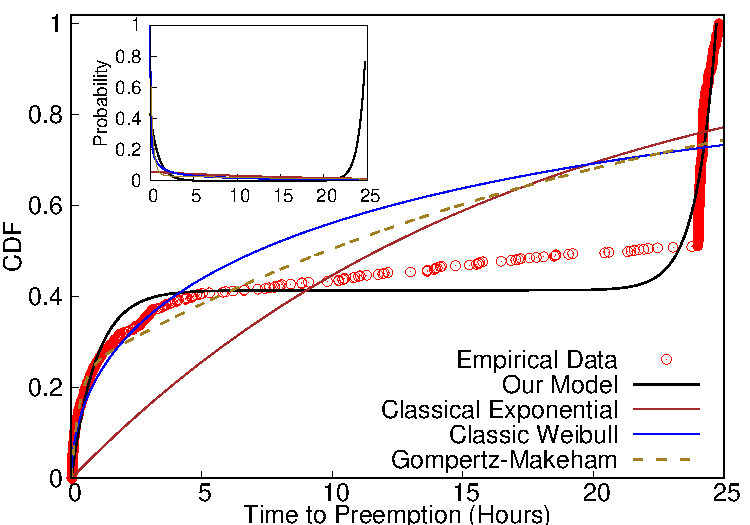
\includegraphics[width=0.44\textwidth]{sigmetrics-fig-cdf-prob-inset-time.pdf} 
  \caption{CDF of lifetimes of Google Preemptible VMs. Our proposed distribution for modeling the constrained preemption dynamics provides a better fit to the empirical data compared to other failure distributions. Inset shows the probability density functions.}
  \label{fig:gcp1}
\end{figure}



\noindent \textbf{Methodology.}
We launched  870 Google Preemptible VMs of different types over a two month period (Feb--April 2019), and measured their time to preemption (i.e., their useful lifetime).
VMs of different resource capacities were launched in four geographical regions; during days and nights and all days of the week; and running different workloads. 
We launched VMs in their default resource configurations (CPU and memory), and do not use custom VM sizes.
To ensure the generality of our empirical observations, VMs were not launched during well-known peak utilization days (such as Black Friday).
The preemption data collection was bootstrapped: a small amount of data points were used to estimate and model the preemption CDF, which we then used to run SciSpot (described and evaluated in Sections~\ref{sec:impl} and \ref{sec:eval}), which generated the rest of the preemption data.  
Due to the relatively high preemption rates compared to EC2 spot instances, we were able to collect these data points for less than \$5,000. 


A sample of over 100 such preemption events are shown in Figure~\ref{fig:gcp1}, which shows cumulative distribution function (CDF) of the lifetime of the \texttt{n1-highcpu-16} VMs in the \texttt{us-east1-b} zone. 
The overall rate of preemptions is ``bathtub'' shaped as shown by the solid black line in the inset of Figure~\ref{fig:gcp1}.
Empirically, our main observations are:


\begin{figure*}
  \subfloat[Preemption characteristics of different VM types. Larger VMs are more likely to be preempted.
  \label{fig:cdf-comparison}]
  {  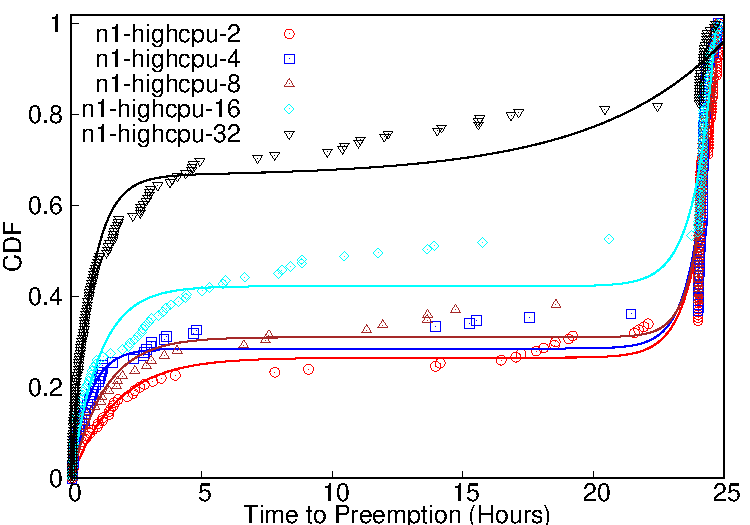
\includegraphics[width=0.3\textwidth]{sigmetrics-fig-vm-types.pdf} }
  \hfill
\subfloat[Variations due to time of day and workload. \label{fig:time-breakdown}]
{  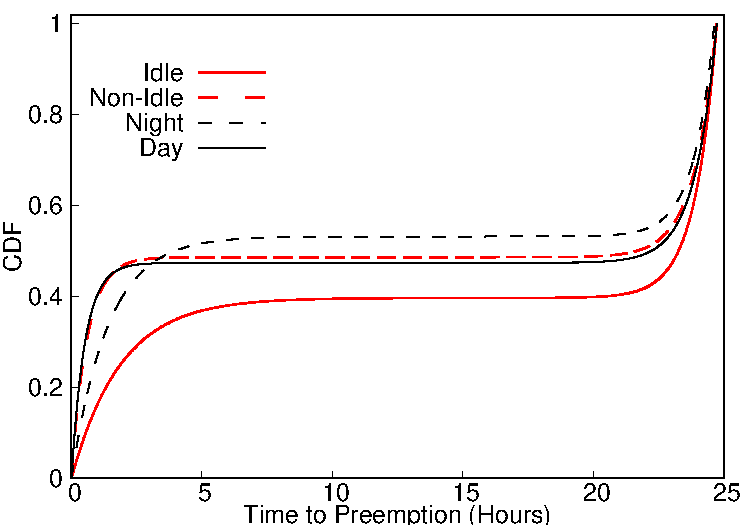
\includegraphics[width=0.3\textwidth]{sigmetrics-time-breakdown.pdf} }
ill
\subfloat[\texttt{n1-highcpu-16} in different regions. \label{fig:region-breakdown}]
{  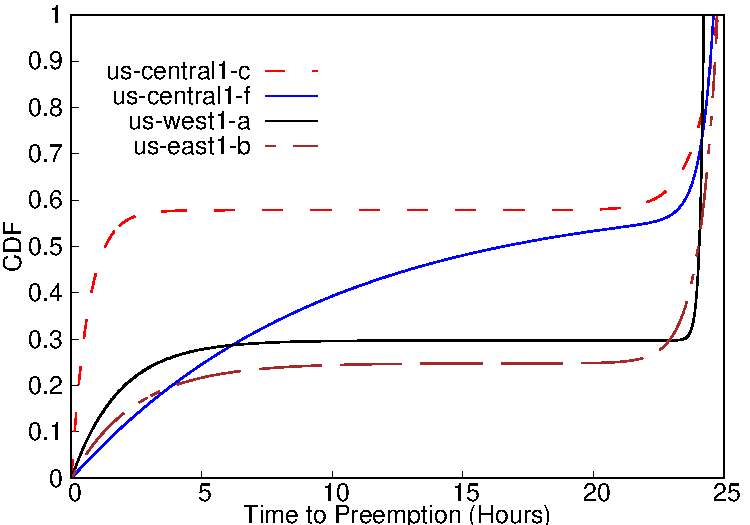
\includegraphics[width=0.3\textwidth]{sigmetrics-region-breakdown.pdf} }
\vspace*{-0.3cm}
\caption{Analysis of preemption characteristics by VM-type, region, time-of-day, and workload type.}
\label{fig:breakdown-all}
    \vspace*{\myfigspace}
\end{figure*}

\begin{figure}
  \centering 
  \subfloat[By day of week. \label{fig:cdf-time}]
  {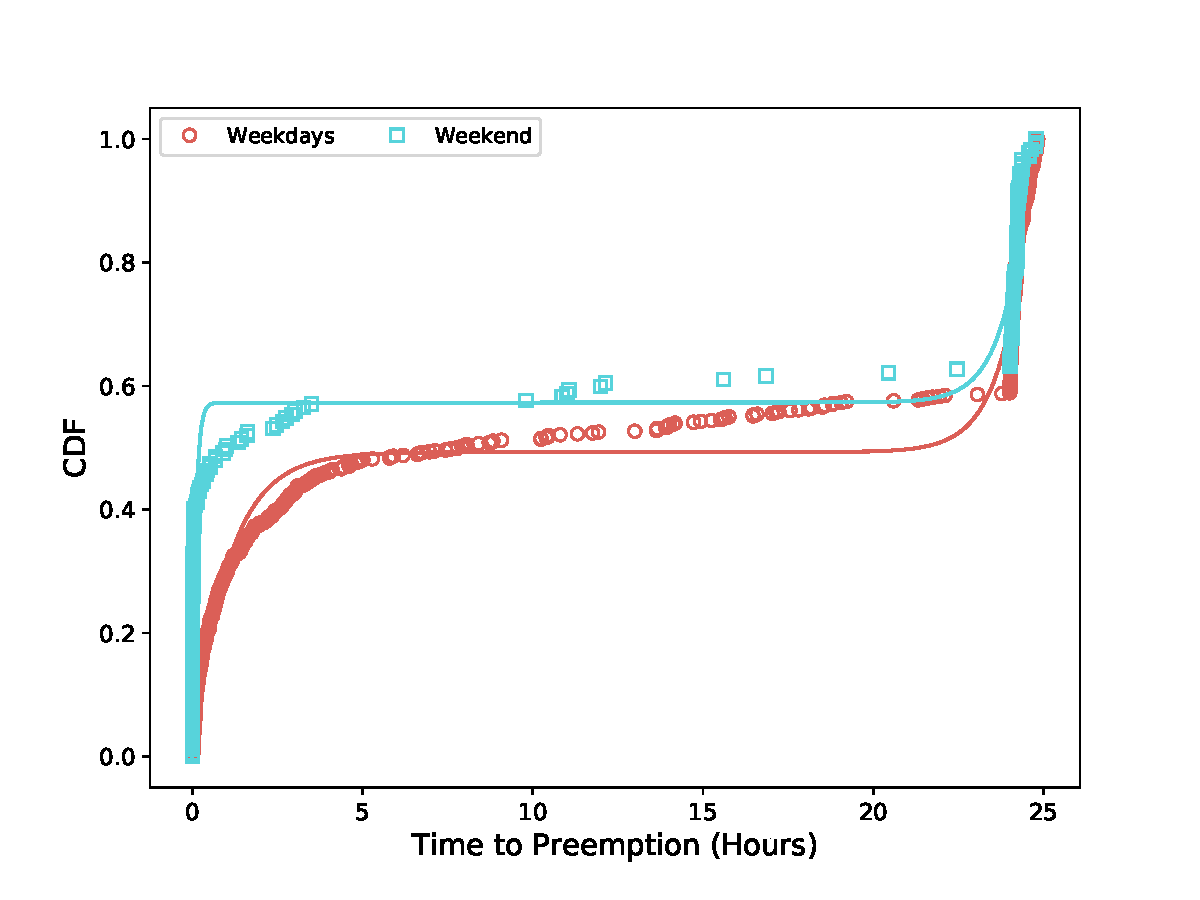
\includegraphics[width=0.34\textwidth]{weekdays-vs-weekends.pdf}}
  \\
  \vspace*{-10pt}
\subfloat[Parallel VM launches. \label{fig:cdf-concurr}]
{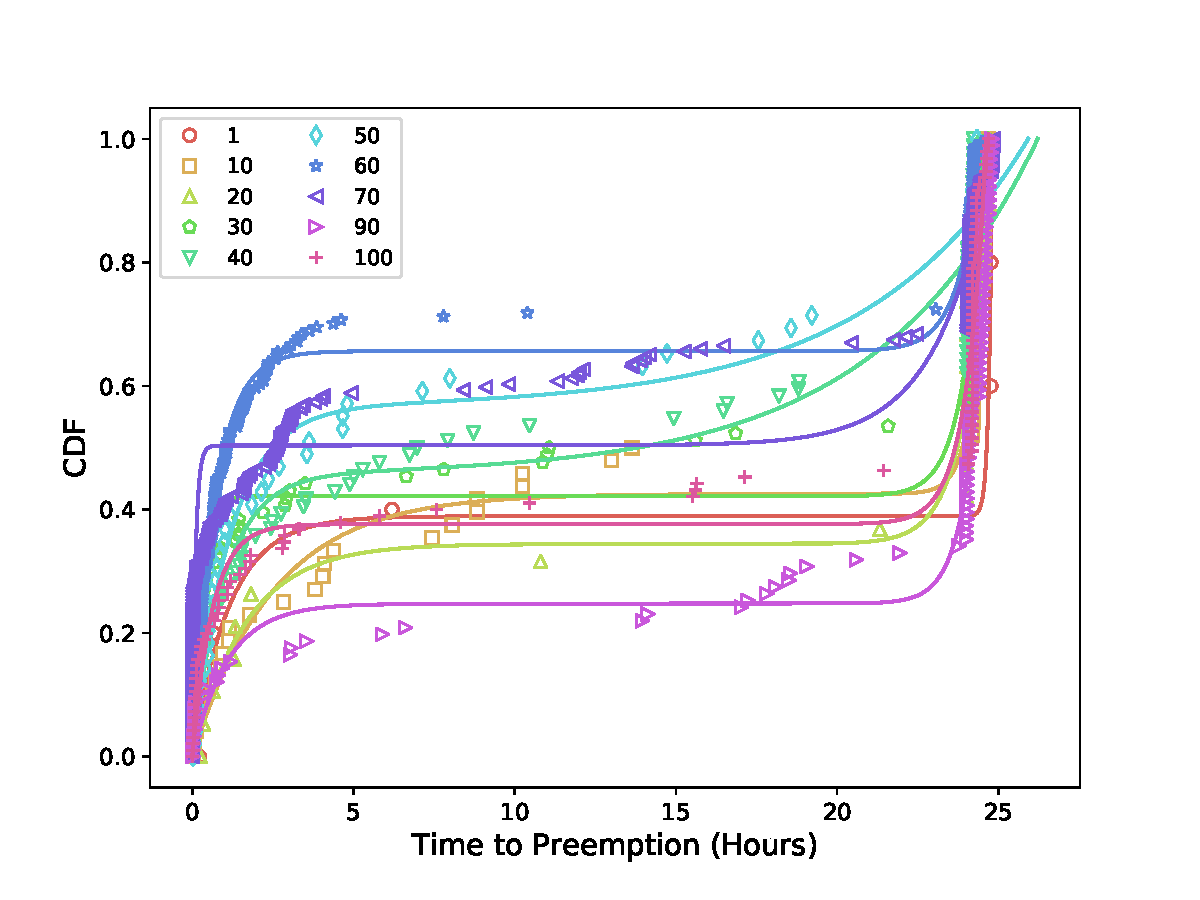
\includegraphics[width=0.34\textwidth]{different-numbers-of-parallel-VM-launches.pdf}}
\label{fig:breakdown-more}
\caption{Preemption CDF analysis.}
\vspace*{-0.3cm}
\end{figure}

\noindent \textbf{Observation 1:} \emph{The lifetimes of VMs are not uniformly distributed, but have three distinct phases.}

\noindent In the first (initial) phase, characterized by VM lifetime $t\in [0, 3]$ hours, we observe that many VMs are quickly preempted after they are launched, and thus have a steep rate of failure. The rate of failure (preemption rate) is the derivative of the CDF.
The early high rate of failure reflects that the cloud service provider takes into account VM liftetime in prioritizing preempting ``younger'' VMs, in other words, the number of simultaneous VMs launched does have an effect on their failure rate. 
In the second phase, VMs that survive past 3 hours enjoy a relatively low preemption rate over a relatively broad range of lifetime (characterized by the slowly rising CDF in Figure~\ref{fig:gcp1}).
The third and final phase exhibits a steep increase in the number of preemptions as the preemption deadline of 24 hours approaches.
The overall rate of preemptions is ``bathtub'' shaped as shown by the solid black line in the inset of Figure~\ref{fig:gcp1} (discussed in detail below).



\noindent \textbf{Observation 2:} \emph{The preemption behavior, imposed by the constraint of the 24 hour lifetime, is substantially different from conventional failure characteristics of hardware components and EC2 spot instances.}

\noindent In ``classical'' reliability analysis, the rate of failure  usually follows an exponential distribution $f(t) = \lambda e^{-\lambda t}$, where $\lambda=1/\text{MTTF}$.
Figure~\ref{fig:gcp1} shows the CDF ($=1-e^{-\lambda t}$) of the exponential distribution when fitted to the observed preemption data, by finding the distribution parameter $\lambda$ that minimizes the least squares error.
The classic exponential distribution is unable to model the observed preemption behavior because it assumes that the rate of preemptions is independent of the lifetime of the VMs, i.e., the preemptions are \emph{memoryless}.
This assumption breaks down when there is a fixed upper bound on the lifetime. 

\noindent \textbf{Observation 3:} \emph{The three preemption phases and associated bathtub shaped preemption probability, can be seen as general characteristics of Preemptible VMs.}

Our empirical study looked at preemptions of VMs of different sizes (Figure~\ref{fig:breakdown-all}a), at different times of the day (Figure~\ref{fig:breakdown-all}b), in different geographical zones (Figure~\ref{fig:breakdown-all}c), and running different workloads.
We also analyzed VMs launched at different days (Figure~\ref{fig:cdf-time}) and also analyzed the effect of concurrent VM launches (Figure~\ref{fig:cdf-concurr}).
In all cases, we find that there are three distinct phases associated with the preemption dynamics giving rise to the bathtub-shaped preemption probability. 


\noindent \textbf{Observation 4:}\emph{ Larger VMs have a higher rate of preemptions.}

Figure~\ref{fig:cdf-comparison} shows the preemption data from five different types of VMs in the Google Cloud \texttt{n1-highcpu-\{2,4,8,16,32\}}, where the number indicates the number of CPUs.
All VMs are running in the \texttt{us-central1-c} zone. 
We see that the larger VMs (16 and 32 CPUs) have a higher probability of preemptions compared to the smaller VMs.
While this could be simply due to higher demand for larger VMs, it can also be explained from a cluster management perspective. 
Larger VMs require more computational resources (such as CPU and memory), and when the supply of resources is low, the cloud operator can quickly reclaim a large amount of resources by preempting larger VMs.
This observed behavior aligns with the guidelines for using preemptible VMs that suggests the use of smaller VMs when possible~\cite{preemptible-documentation}. 

\noindent \textbf{Observation 5:} \emph{Preemptions exhibit diurnal variations, and are also affected by the workload inside the VM.}

From Figure~\ref{fig:time-breakdown}, we can see that VMs have a slightly longer lifetime during the night (8 PM to 8 AM) than during the day\footnotemark. 
This is expected because fundamentally, the preemption rates are higher during periods of higher demand. 
We also notice that completely idle VMs have longer lifetimes than VMs running some workload, presumably because idle VMs are easier for resource overcommittment~\cite{sharma19eurosys, fuerst2020cloud}, and thus have a lower preemption probability. 


\footnotetext{Time-zone local to the VM's location.}






\noindent \textbf{Significance of bathtub preemptions.} 
The bathtub shaped preemption distribution is not a coincidence.
It is a result of fundamental characteristics of constrained preemptions that benefit applications. 
For applications that do not incorporate explicit fault-tolerance (such as checkpointing), early preemptions result in less wasted work than if the preemptions were uniformly distributed over the 24 hour interval.
Furthermore, the low rate of preemptions in the middle periods allows jobs that are smaller than 24 hours to finish execution with only a low probability of failure, once they survive the initial preemption phase. 
We compare application performance with bathtub preemptions and uniformly distributed preemptions later in Section~\ref{sec:eval}, and find that bathtub preemptions can reduce the performance overheads of preemptions by up to $10\times$.
However, effective policies for constrained preemptions  require a probability model of preemptions, which must incorporate the temporal constraint and the steep bathtub behavior. 
Existing preemption models are not applicable, and we present our new model next. 






\vspace*{\subsecspace}
\subsection{Failure Probability Model}
\label{subsec:analytical-model}

We now develop an analytical probability model for finding a preemption at a given time that is faithful to the empirically observed data and provides a basis for developing running-time and cost-minimizing optimizations. 
Modeling the dynamics of preemptions constrained by a finite deadline raises many challenges for existing preemption models that have been used for other transient servers such as EC2 spot instances.
We first discuss why existing approaches to preemption modeling are not adequate, and then present our probability model and associated reliability theory connections. 





\vspace*{\subsecspace}
\subsubsection{Our  model}
\label{subsec:preemption-model}



Our failure probability model seeks to address the drawbacks of existing reliability theory models for modeling constrained preemptions. 
The presence of three distinct phases exhibiting non-differentiable transition points (sudden changes in CDF near the deadline, for example) suggests that for accurate results, models that treat the probability as a step function (CDF as a piecewise-continuous function) could be employed.
However, this limits the range of model applicability and general interpretability of the underlying preemption behavior. Our goal is to provide a broadly applicable, continuously differentiable, and informative model built on reasonable assumptions.  


We begin by making a key assumption: the preemption behavior arises from the presence of \emph{two} distinct failure processes.
The first process dominates over the initial temporal phase and yields the classic exponential distribution that captures the high rate of early preemptions.
The second process dominates over the final phase near the 24 hour maximum VM lifetime and is assumed to be characterized by an exponential term that captures the sharp rise in preemptions that results from this constrained lifetime. 


Based on these observations, we propose the following general form for the CDF:

\vspace*{\subsecspace}
\begin{equation}
  \label{eq:blend1}
  \boxed{
  F\left(t\right) = A\left(1-e^{-\frac{t}{\tau_1}} + e^{\frac{t-b}{\tau_2}}\right)}
  \end{equation}
\noindent where $t$ is the time to preemption, $1/\tau_1$ is the rate of preemptions in the initial phase, $1/\tau_2$ is the rate of preemptions in the final phase, $b$ denotes the time that characterizes ``activation'' of the final phase where preemptions occur at a very high rate, and $A$ is a scaling constant. 
The model is fit to data for $0 < t < L$, where $L \approx 24$ hours represents the temporal interval (deadline).
Combination of the 4 fit parameters ($\tau_1, \tau_2, b$, and $A$) are chosen to ensure that boundary condition $F(0) \approx 0$ is satisfied.
In practice, typical fit values yield $b \approx 24$ hours, $\tau_1 \in [0.5, 1,5] $, $\tau_2 \approx 0.8$, and $A \in [0.4, 0.5]$.






For most of its life, a VM sees failures according to the classic exponential distribution with failure-rate equal to $1/\tau_1$ -- this behavior is captured by the $1-e^{-t/\tau_1}$ term in Equation~\ref{eq:blend1}. 
As VMs get closer to their maximum lifetime imposed by the cloud operator, they are reclaimed (i.e., preempted) at a high rate $1/\tau_2$, which is captured by the second exponential term, $e^{(t-b)/\tau_2}$ of Equation~\ref{eq:blend1}. 
Shifting the argument ($t$) of this term by $b$ ensures that the exponential reclamation is only applicable near the end of the VM's maximum lifetime and does not dominate over the entire temporal range. 


The analytical model and the associated  distribution function $\mathscr{F}$ introduced above provides a much better fit to the empirical data (Figure~\ref{fig:gcp1}) compared to other models, and captures the different phases of the preemption dynamics through parameters $\tau_1, \tau_2, b$, and $A$. These parameters can be obtained for a given empirical CDF using least squares function fitting methods (we use scipy's \texttt{optimize.curve\_fit} with the dogbox technique~\cite{scipy-fit}). The failure or preemption rate can be derived from the CDF in Equation \ref{eq:blend1} as:
\begin{equation}
  \label{eq:failrate}
    \vspace*{\eqnspace}
f(t) = \dfrac{d F(t)} {dt} = A \left(\dfrac{1}{\tau_1}e^{-t/\tau_1} + \dfrac{1}{\tau_2}e^{\frac{t-b}{\tau_2}}\right).
\end{equation}
$f(t)$ vs. $t$ yields a bathtub type failure rate function for the associated fit parameters (inset of Figure~\ref{fig:gcp1}).






\subsubsection{Reliability Analysis}
\label{subsec:reliability}

We now analyze and place our model in a reliability theory framework. 

\noindent \textbf{Expected Lifetime.} Our analytical model helps crystallize the differences in VM preemption dynamics, by allowing us to easily calculate their expected lifetime. 
More formally, we define the expected lifetime of a VM ($\mathscr{L}$) as: 
\begin{equation}
  \label{eq:expected-lifetime}
E[\mathscr{L}] =  \int_{0}^{L} t {f}(t)~dt =  -A(t+\tau_1)e^{-t/\tau_1} + A(t-\tau_2) e^{\frac{t-b}{\tau_2}} \biggr\rvert_{0}^{L}
\end{equation}
where $f(t)$ is the rate of preemptions of the VM (Equation~\ref{eq:failrate}).
This expected lifetime can be used in lieu of MTTF, for policies and applications that require a ``coarse-grained'' comparison of the preemption rates of servers of different types, which has been used for cost-minimizing server selection~\cite{flint}. 


\noindent \textbf{Hazard Rate.}
The hazard rate $\lambda(t)$ governs the dynamics of the failure (or survival) processes. It is generally defined as $\lambda(t) = \frac{f(t)}{S(t)}$ and often expressed via the following differential equation (rate law):
\begin{equation}\label{eq:hazard}
\frac{dS(t)}{dt} = -\lambda(t) S(t),
\end{equation}
where $S(t) = 1 - F(t)$ is the survival function associated with a CDF $F(t)$, and $f(t)=dF(t)/dt$ is the failure probability function (rate) at time $t$. The survival function indicates the amount of VMs that have survived at time $t$.
The hazard rate can also be directly expressed in terms of the CDF as follows: $1-F(t) = \exp{\int_0^t{-\lambda(x) ~dx}}$. 
The exponential distribution has a constant hazard rate $\lambda$.
The Gompertz-Makeham distribution has an increasing failure rate to account for the increase in mortality, and its hazard rate is accordingly time-dependent and given by $\lambda(t) = \lambda + \alpha e^{\beta t}$.

Since we model multiple failure rates and deadline-induced preemptions, our hazard rate is expected to increase with time. Defining the survival function for our model: $S = 1 - F$, and using Eq.~\ref{eq:hazard} yields the hazard rate associated with our model: 
\noindent 
\begin{equation}
  \label{eq:hmodel}
  \lambda 
  = \dfrac{r_1 e^{- r_1 t} + r_2 e^{r_2 (t - b)}}{1/A - 1 + e^{- r_1 t} - e^{r_2 (t - b)}}
\end{equation}
where we have introduced $r_1 = 1/\tau_1$, $r_2 = 1/\tau_2$ to denote the rates of preemptions associated with initial and final phases respectively.




Recall that the sharp increase in preemption rate only happens close to the deadline, which means that $b \lesssim L$. Thus, when $0 < t \ll b$, we get $\lambda(t) \approx r_1$, mimicking the hazard rate for the classic exponential distribution.
As $t$ approaches and exceeds $b$ (i.e., $b\lesssim t < L$), the increase in the hazard rate due to the second failure process kicks in, accounting for the deadline-induced rise in preemptions. Note that our hazard rate satisfies $\lambda(t) \ge 0$ for $0<t<L$.





\subsection{Statistical mechanics of constrained preemptions}
\label{subsec:stat-mech}

For constrained preemptions, one might expect to see uniformly distributed preemptions with a probability $1/L$ over $[0, L]$. 
However, as our empirical analysis shows, the preemption distribution is bathtub-shaped.
Interestingly, we can show using exact analytical arguments that non-uniform, bathtub distributions are in fact an \emph{emergent} characteristic of systems with constrained preemptions, modulo some assumptions. 

\begin{lemma}\label{lemma:1}
  Consider $N$ randomly distributed preemptions over an interval $[0, L]$.
  Assume that each preemption takes $w > 0$ time-units to perform, and preemptions cannot overlap, i.e, they occur in a mutually exclusive manner.
  Then, there exists $\epsilon > 0$ such that  $P(L-\epsilon) > \frac{1}{L}$, where 
 $P(t)$ is the probability of finding a preemption at time $t$. 
\end{lemma}


\begin{proof} 
We first make some preliminary remarks and introduce concepts necessary to complete the proof. 

Firstly, mutual exclusion of preemptions implies that there is a finite non-zero waiting time $w>0$ between preemptions. 
For $N$ preemptions to occur within $L$ interval, evidently, we must have $N w < L$. Also, while $w >0$, the time to perform the preemption is generally expected to be much smaller than the total time interval $L$ (i.e., $w \ll L$).
$N$ preemptions occupy a ``temporal volume'' of $Nw$ (volume here represents the one-dimensional volume). We assume that while a preemption may start at $t=0$, the last preemption must finish by $t = L$. Thus, the amount of free or excluded ``temporal volume'' available within the constrained system is $L_e = L - w - (N-1)w = L - Nw$.
We note that the concept of excluded volume is routinely employed in the analysis of physical systems such as liquids and polymers, where the excluded volume of particles acts as a constraint that gives rise to steric forces and structural changes in material behavior \cite{krauth2006statistical,jing2015ionic,solis2013generating}. 

Secondly, we observe that the system of $N$ preemptions within a constrained deadline of interval $L$ maps \emph{exactly} to a well known and analytically solvable system in classical statistical mechanics, the one-dimensional Tonks gas model \cite{tonks}. The Tonks gas model describes a system of $N$ non-overlapping particles of finite size $w$ that are constrained to move within a line segment of length $L$. The structural quantities associated with this system, including the probability of finding a particle at position $x$ within the spatial confinement of length $L$, are computed by evaluating the partition function of the system, which essentially measures the number of valid system configurations \cite{krauth2006statistical}. 
Employing this mapping, we consider a system of $N$ non-overlapping preemptions constrained within a ``time confinement'' of size $L$. Each preemption has access to an excluded volume of $L_e$ within this constrained system. 
The number of ways $N$ preemptions can occur within the interval $L$ is equivalent to the number of valid configurations for this system, which is given by its partition function: $Z_N = L_e^N = (L- Nw)^N$.

We are interested in calculating the probability that a preemption starts at time $t=L-w$, i.e., $P(L-w)$. Given $w \ll L$, $P(L-w)$ is the probability of finding a preemption near the deadline. The assumption of mutually exclusive preemptions implies that no other preemption can be found for $t > L - w$, that is, $P(t> L-w) = 0$. Hence, the remaining $N-1$ preemptions must occur such that the last of those finish by $t=L-w$. In other words, the preemption at time $L-w$ essentially sets an effective deadline for the other $N-1$ preemptions. The number of ways those $N-1$ preemptions can happen within the time interval of $L-w$ is given by the partition function $Z_{N-1} = L_e^{N-1}= (L-2w - (N-2)w)^{N-1} = (L - Nw)^{N-1}$, where $L_e = L - Nw$ is the corresponding excluded temporal volume available to each of the $N-1$ preemptions.
It is interesting to note that this excluded volume
is the same as that of the original $N$ preemption system: this fortuitous result arises because the decrease in the available volume (``time confinement'') to place the preemptions is commensurate with the need to place fewer ($N-1$) preemptions.

The probability $P(L-w)$ is obtained as the ratio of the valid configurations given by the two partition functions computed above.
That is, $P(L-w) = Z_{N-1}/ {Z_N} = \frac{1}{L - Nw}$. Because $N \geq 1$ and $w>0$, we find $P(L-w) > \frac{1}{L}$. Choosing $\epsilon = w$ completes the proof.
\end{proof}

By symmetry arguments, the above lemma is in fact valid for both the end points of the interval, i.e., $P(\epsilon) > \frac{1}{L}$.
In other words, the probability of preemption is higher near the end points (deadline) than the average preemption probability of $1/L$, and we get a bathtub shaped distribution.
For the above proof, we assumed that each preemption event occurs over a timespan of $w$, which is determined by the preemption warning that the cloud platform provides (which is 30 seconds for Google Preemptible VMs and 120 seconds for Amazon EC2 spot instances). 
Preempting a VM and reclaiming its resources involves manipulating the cluster-management state, and mutually exclusive preemptions may be convenient for cluster management, since serializing VM preemptions makes accounting and other cluster operations easier.
From an application standpoint, non-overlapping preemptions are also beneficial, since handling multiple concurrent preemptions is significantly more challenging~\cite{exosphere}. 



Thus, statistical mechanics indicates that the bathtub distribution follows from the constrained and non-overlapping nature of preemptions, if we assume no other external factors or cloud policies influencing the preemptions. 
Figure~\ref{fig:partfun} shows the preemption probability computed using the partition function.
We find that this probability \emph{also} follows the bathtub shape that is found in the empirical data. 




\begin{figure}[t]
  \centering
  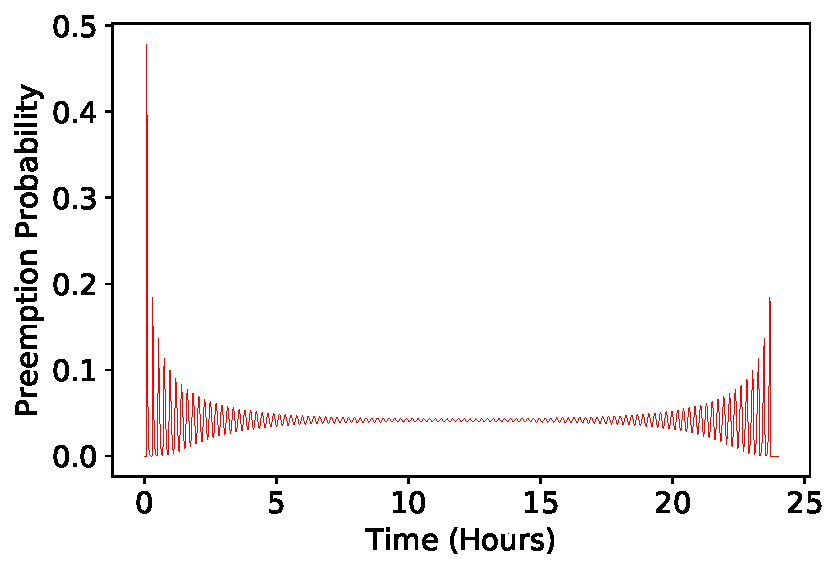
\includegraphics[width=0.3\textwidth]{analytical_prob.pdf}
  \caption{Preemption probability computed using the partition function defined for a simple constrained system is also bathtub shaped.}
  \label{fig:partfun}
\end{figure}



\subsection{Model Validity and Generalizability}

In the absence of any prior work on constrained preemption dynamics, our aim is to provide an interpretable model with a minimal number of parameters, that provides a sufficiently accurate characterization of features present in the preemption data. 
Extension of this model to include more failure processes would introduce more parameters and reduce the generalization power. Further, this model as well as the optimization policies derived from it offer pathways to quantify additional effects arising due to the inclusion of more failure processes.  

In Section~\ref{subsec:eval-sched}, we  show that constant failure rate assumptions can be severely detrimental to the application failures and performance. 
We show that our bathtub model, \emph{even with poorly fitted parameters}, can provide significant improvement in job running times, compared to existing exponential models.



 



































 
\vspace*{\subsecspace}
\section{Policies For Ameliorating Constrained Preemptions}
\label{sec:policies}
Having analyzed the statistical behavior of constrained preemptions and presented our probability model, we now examine how the bathtub shape of the failure rate impacts applications. 
Based on insights drawn from our statistical analysis and the model, we develop various policies for ameliorating the effects of preemptions. 
Prior work in transient computing has established the benefits of such policies for a broad range of applications. 
However, the constrained nature of preemptions introduces new challenges that do not arise in other transient computing environments such as Amazon EC2 spot instances, and thus new approaches are required. 
In this section, we first analyze the impact of constrained preemptions on job running time, and then develop new constrained-preemption aware policies for job scheduling and cost optimization. 


\noindent \textbf{Workload Assumptions.}
Our primary focus is on long-running batch jobs that arise in many scientific computing applications. 
Our scheduling policy assumes that \emph{approximate} job running times are known: which is often the case with ``bags of jobs'', as described in the next section. 
Specifically, we only require knowledge of whether the job running time is above or below a threshold.









\vspace*{\subsecspace}
\subsection{Job Running Time Modeling}

SciSpot uses our bathtub probability model to predict the total running time (i.e., the makespan) of the job. 
When a preemption occurs during the job's execution, it results in wasted work, assuming there is no checkpointing. 
This increases the job's total expected running time, since it must restart after a preemption.
The expected wasted work depends on two factors:
\begin{enumerate} [leftmargin=12pt]
\item The probability of the job being preempted during its execution. 
\item \emph{When} the preemption occurs during the execution. 
\end{enumerate}

We can analyze the wasted work due to a preemption using the failure probability model.
We first compute the expected amount of wasted work \emph{assuming} the job faces a single preemption, which we denote by $E[W_1(T)]$, where $T$ is the original job running time (without preemptions):
\begin{equation}
E[W_1(T)] = \int_0^{T} t~P(t | t \leq T)~dt.
\end{equation}
Here, $P(t|t\leq T) = P(t) / P(t \leq T)$. $P(t\leq T)$ is the probability that there is a preemption within time $T$ and is given by $P(t \leq T) = F(T)$, where $F(T)$ is the CDF (Equation \ref{eq:blend1}). 
$P(t)$ is the probability of a preemption at time $t$, and is given by $P(t) = f(t)$, where $f(t)$ is the preemption rate (Equation~\ref{eq:failrate}).
We can therefore write the above equation as:
\begin{equation}
  E[W_1(T)] = \int_0^{T} t~P(t | t \leq T)~dt = \frac{1}{F(T)}  \int_0^{T} t~f(t)~dt.
    \label{eq:wasted}
\end{equation}

We note that the integral is the same as the ``expected lifetime'', given by Equation~\ref{eq:expected-lifetime}.
The above expression for the expected waste due to a single preemption can be used by users and application frameworks to estimate the increase in running time due to preemptions. 
The total running time (also known as makespan) of a job \emph{with} preemptions is given by:
\begin{equation}
  \label{eq:tot-run-time}
  E[T] = P(\text{no failure})~T + P(\text{1 failure})~\left(T + E[W_1(T)]\right),
\end{equation}
where $P(\text{no failure}) = P(t > T) =  1- F(T)$ and $P(\text{1 failure}) = P(t \leq T) = F(T)$.
Expanding out these terms and using Equation \ref{eq:wasted}, we get
\begin{align}
  \label{eq:tot-run-time-2}
  E[T] &= \left(1-F\left(T\right)\right)T + F(T)\left(T + E[W_1(T)]\right) \notag \\
  &= T + \int_0^{T} t~f(t)~dt.         
\end{align}
This expression for the expected running time assumes that the job will be preempted at most once.
An expression which considers multiple ($>1$) job failures easily follows from this base case, but presents relatively low practical value.



\noindent \textbf{Consequences for applications.}
Based on our analysis, both the increase in wasted time ($E[W_1(T)]/T$) and expected running time $(E[T]/T)$ depend on the length of the job for non-memoryless constrained preemptions. 
For memoryless exponential distributions, the expected waste is simply $T/2$, but this assumption is not valid for constrained preemptions, and thus job lengths must be considered when evaluating the suitability of Preemptible VMs. 


Users and transient computing systems can use the expected running time analysis for scheduling and monitoring purposes.
Since the preemption characteristics are dependent on the type of the VM and temporal effects, this analysis also allows principled \emph{selection} of VM types for jobs of a given length. 
For instance, VMs having a higher initial rate of preemptions are particularly detrimental for short jobs, because the jobs will see high rate of failure and are not long enough to run during the VM's stable period with low  preemption rates. 
We evaluate the expected wasted time and running time for Google Preemptible VMs later in Section~\ref{sec:eval}. 

\vspace*{\subsecspace}
\subsection{Transition-Points based Job Scheduling and VM Reuse Policy}
\label{subsec:sched-policy}

Our bathtub probability model also allows us to develop optimized job-scheduling policies for \emph{reducing} job-failures in the bag of jobs execution model. 
In the case of deadline-constrained bathtub preemptions, we face a choice: we can either run a new job on an already running VM, or relinquish the VM and run the job on a \emph{new} VM. 
This choice is important in the case of non-uniform failure rates, since the job's failure probability depends on the ``age'' of the VM. 
Because of the bathtub failure distribution, VMs enjoy a long period of low failure rates during the middle of their total lifespan.
Thus, it is beneficial to \emph{reuse} VMs for multiple jobs, and relinquishing VMs after every job completion may not be an optimal choice. 


However, jobs launched towards the end of VM life face a tradeoff.
While they may start during periods of low failure rate, the 24 hour deadline-imposed sharp increase in preemptions poses a high risk of preemptions, especially for longer jobs.
The alternative is to discard the VM and run the job on a new VM. 
However, since newly launched VMs also have high preemption rates (and thus high job failure probability), the choice of running the job on an existing VM vs. a new VM is not obvious. 

Our job scheduling policy uses the preemption model to determine the preemption probability of jobs of a given length $T$. 
Assume that the running VM's age (time since launch) is $s$.
The intuition is to reuse the VM only if the expected running time is lower, compared to running on a new VM. 
To compute the expected running time of a job of length $T$ starting at vm-age $s$, we  modify our earlier expression for running time (Equation~\ref{eq:tot-run-time-2}) to: 
\begin{equation}
  \label{eq:tot-run-time-s}
    E[T_s]  = T + \int_{s}^{s+T} t~f(t)~dt
  \end{equation}
The alternative is to discard the VM and launch a new VM, in which case the expected running time is $E[T_0]$. Our job-scheduling policy is simple: 
When a job of running time $T$ attempts to start on a VM of age $s$, if $E[T_s] \leq E[T_0]$, then we run the job on the existing VM.
Otherwise, a new VM is launched.









\noindent \textbf{Transition Points Policy.}
SciSpot builds on the above insight and determines the job-scheduling and VM-reuse decision. 
Based on different job lengths within a bag of jobs and the age of the VM, we minimize the total expected running time of a job.
For any job running time (T), and VM age (s), we compute  $\delta(s,T) = E[T_s] - E[T]$.
If $\delta(s,T) \geq 0$, then a new VM is used, as illustrated in Figure~\ref{fig:transition-example}.


Figure~\ref{fig:transition-example} shows that reusing VMs is preferred for shorter job lengths, and the range of jobs for which reusing is good depends on the current age of the VM: younger VMs ($s=1$ hour) can be used for longer job lengths compared to older VMs. 
For a given VM type, we precompute this function for different $(s, T)$ values, and find the transition points where launching a new VM is suitable. 
The precomputed $\delta(s,T)$ can be seen in Figure~\ref{fig:transition-boundary}.
We \emph{analytically} compute the transition point ``frontier'' which is deliniates the re-use vs. new VM portion of the figure. 
Given the VM age $s$, we only need to determine whether the job length is greater or smaller than the transition point. 
This policy has the practical advantage that accurate job running times are not needed---we only require running times relative to the transition point. 
Using this figure, SciSpot, and users in general, can simply lookup the job and VM attributes, and determine the optimal decision. 




\begin{figure}[t]
  \subfloat[Difference in expected running times vs. job length $T$ for different VM age $s$. All times are in hours. \label{fig:transition-example}]
  {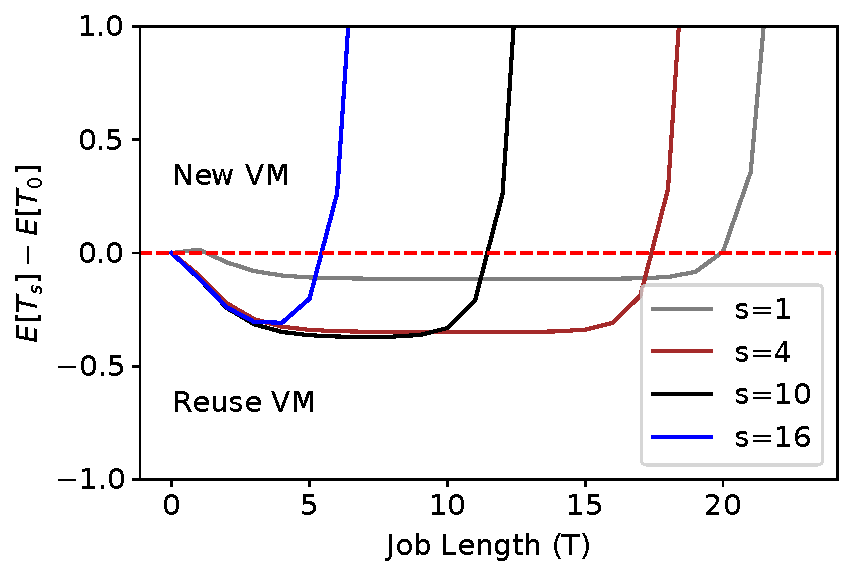
\includegraphics[width=0.26\textwidth]{transition-all.pdf}}
  \hfill
  \subfloat[Transition boundary depends on job length and when the job starts on the VM. \label{fig:transition-boundary}]
  {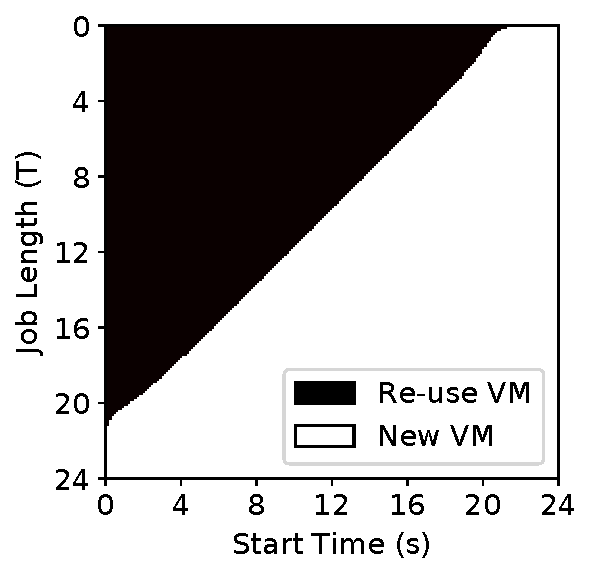
\includegraphics[width=0.2\textwidth]{tipping.pdf}}
  \label{fig:transition-all}
  \caption{Reusing vs. running on a new VM.}
\end{figure}






\subsection{Cost-aware VM Selection}
\label{subsec:vm-selection}

VM-selection is an important optimization in cloud environments, because VMs have different tradeoffs of cost, performance, and preemption characteristics. 
Application performance is affected by the size of the VM (due to network communication and parallel scaling overheads), and the preemption rates. 
Our policy selects the ``right'' type of  VMs that minimizes the expected job failure probability and cost by using the analytical preemption models. 






We assume that the total resource requirement for a job, $\mathcal{R}$, is provided by the user based on prior speedup data, the user's cloud budget, and the deadline for job completion.
Assume that the cloud provider offers $N$ server types, with the price (per unit time) of a server type equal to $c_i$. 
The overall expected cost of running a job is: 
\begin{equation}
  \label{eq:e-cost}
\vspace*{\eqnspace}
  E[C_{( i,n_i )}] = n_i\times c_i \times E[\mathcal{T}_{( i,n_i )}].
\end{equation}
Here, $E[\mathcal{T}_{( i,n_i )}]$ denotes the expected makespan of the job (accounting for preemptions) on $n_i$ servers of type $i$. 
This turnaround time depends on whether the job needs to be recomputed because of preemptions, and is given by Equation~\ref{eq:tot-run-time-2}. 
\sysname searches over all available and acceptable VM types (modulo any resource constraints on minimum memory/CPUs/GPUs), and picks the VM type which yields the lowest expected cost.
The search process is aided by the bag of jobs abstraction: initial jobs are used for determining the lowest-cost VM, on which the remaining jobs are run. 









 


\section{SciSpot Design and Implementation}
\label{sec:impl}

We have developed \sysname as a prototype batch computing service that implements various policies for constrained preemptions. 
We use it to examine the effectiveness and practical utility of our model and policies in real-world settings. 
\sysname is implemented as a light-weight, extensible framework that makes it convenient and cheap to run batch jobs in the cloud. 
We have implemented our prototype in Python in about 2,000 lines of code, and currently support running VMs on the Google Cloud Platform~\cite{gcp}. 


We use a centralized controller (Figure~\ref{fig:arch}), which implements the VM selection and job scheduling policies described in Section~\ref{sec:policies}. 
The controller can run on any machine (including the user's local machine, or inside a cloud VM), and exposes an HTTP API to end-users. 
Users submit either a bag or individual jobs to the controller via the HTTP API, which then launches and maintains a cluster of cloud VMs, and maintains the job queue and metadata in a local database. 

\sysname integrates, and interfaces with two primary services.
First, it uses the Google cloud API~\cite{gcloud-api} for launching, terminating, and monitoring VMs.
Once a cluster is launched, it then configures a cluster manager such as Slurm~\cite{slurm} or Torque~\cite{torque}, to which it submits jobs. 
\sysname uses the Slurm cluster manager, with each VM acting as a Slurm ``cloud'' node, which allows Slurm to gracefully handle VM preemptions.
The Slurm master node runs on a small, 2 CPU non-preemptible VM, which is shared by all applications and users. 
We monitor job completions and failures (due to VM preemptions) through the use of Slurm call-backs, which issue HTTP requests back to the central service controller. 

\noindent \textbf{Policy Implementation.}
\sysname creates and manages clusters of transient cloud servers, manages all aspects of the VM lifecycle and costs, and implements the model-based policies.
It manages a cluster of VMs, and parameterizes the bathtub model based on the VM type, region,  time-of-day, and day-of-week.
When a new batch job is to be launched, \sysname finds a ``free'' VM in the cluster that is idle, and uses the job scheduling policy to determine if the VM is suitable or a new VM must be launched. 
Due to the bathtub nature of the failure rate, VMs that have survived the initial failures are ``stable'' and have a very low rate of failure, and thus are ``valuable''.
We keep these stable VMs as ``hot spares'' instead of terminating them, for a period of one hour. 



\begin{figure}[t]
  \centering 
  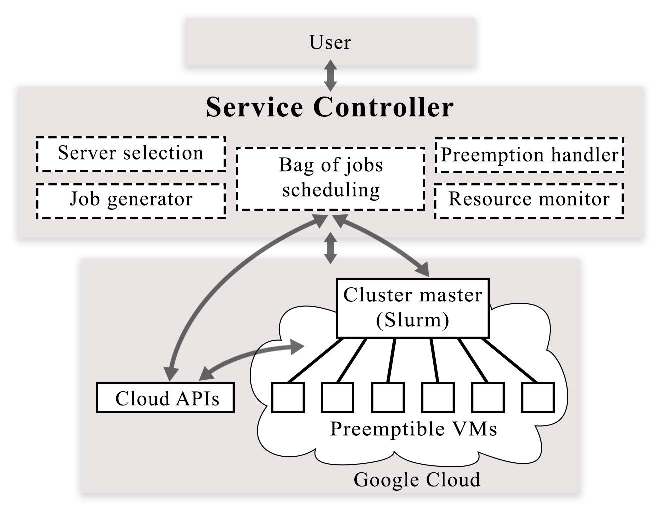
\includegraphics[width=0.3\textwidth]{ArchitectureRevisedV2.pdf}
\vspace*{\myfigspace}
  \caption{Architecture and system components of SciSpot.}
  \label{fig:arch}
  \vspace*{\myfigspace}
\end{figure}


\noindent \textbf{Bag of Jobs Abstraction For Scientific Simulations.}
While \sysname is intended for general batch jobs, we incorporate a special optimization for scientific simulation workloads that improves ease-of-use, and also helps in our policy implementation. 
Our insight is that many scientific simulations involve launching a series of jobs that explore a large parameter space that results from different combinations of physical and computational parameters.
These workloads can be abstracted as a ``bag of jobs'', with each job running the same application with  different parameters.
Bags of jobs are increasingly common in emerging applications that combine Machine Learning (ML) techniques with scientific simulations to enhance the predictive power or reduce the
computational costs of  simulations~\cite{ferguson2017machine,wang2019machine,casalino2021ai,kadupitiya2020machine,kadupitiya2020machine2}. 

We allow users to submit entire bags of jobs, which permits us to estimate the running time of jobs based on previous jobs in the bag.
These running time estimates can then be used for the transition-points based policy described in Section~\ref{subsec:sched-policy}. 

Having a large sequence of jobs is also particularly useful with bathtub-shaped preemption rates, because we can re-use ``stable'' VMs with low preemption probability for running new jobs from a bag.
Thus, SciSpot maintains a pool of these idle VMs as hot-spares. 
Idle VMs are retained for one hour. 






















 
\vspace*{\subsecspace}
\section{SciSpot Experimental Evaluation}
\label{sec:eval}



In this section, we present analytical and empirical evaluation of \sysname.
We have already presented the statistical analysis of our model in Section~\ref{sec:failmodel}, and we now focus on answering the following questions: 

\begin{enumerate}
\item How do constrained preemptions impact the total running time of applications?

\item  What is the effect of our model-based policies when compared to existing transient computing approaches?


\item What is the cost and performance of \sysname for real-world workloads? 
  
\end{enumerate}


\noindent \textbf{Environment and Workloads:}
All our empirical evaluation is conducted on the Google Cloud Platform using our batch computing service described in Section~\ref{sec:impl}. 
All the experiments are conducted in the same time period, and have the same preemption characteristics, as described in our data collection methodology in  Section~\ref{sec:failmodel}.
We ran more than 800 VMs running different bags of jobs in a ``closed-loop'' manner, such that SciSpot always launched a replacement VM to replenish preempted VMs.
Since most bags of jobs take several hours to run, this gave us good temporal coverage of VM launches.
All VMs of a bag of jobs were either run in the \texttt{us-east1-b} or the  \texttt{us-central1-c} region. 

We run each workload atleast five times and report the average running times and costs. 
We use three scientific computing workloads that are representative of  applications in the broad domains of physics and materials science:


\noindent \textbf{Nanoconfinement.}
The nanoconfinement application launches molecular dynamics (MD) simulations of ions in nanoscale confinement created by material surfaces \cite{jing2015ionic,kadupitiya2017,anousheh2020ionic}. The running time is 14 minutes on a 64 CPU core cluster (4 n1-highcpu-16 VMs). 

\noindent \textbf{Shapes.} The Shapes application runs an MD-based simulated annealing procedure to predict the optimal shape of deformable nanoparticles \cite{jto1,brunk2019computational,brunk2020}. The running time is 9 minutes on a 64 CPU core cluster (4 n1-highcpu-16 VMs). 

\noindent \textbf{LULESH.} Livermore Unstructured Lagrangian Explicit Shock Hydrodynamics (LULESH) is a popular benchmark 
for hydrodynamics simulations of continuum models of materials~\cite{IPDPS13:LULESH,LULESH2:changes}. The running time is 12.5 minutes on 8 n1-highcpu-8 VMs.










Wherever applicable, we compare against policies designed for EC2 spot instances~\cite{harlap2018tributary, spoton} that have memoryless preemptions.
Specifically, we compare against the policies of ExoSphere~\cite{exosphere}, which is a state of the art system for EC2 spot instances, and uses portfolio-theory to minimize application revocations and cost.
We ported its policies to use SciSpot's preemption model---specifically, ExoSphere requires the MTTFs of all VM types. 
However, we also note that certain resource management challenges such as the preemption-rate aware job scheduling are \emph{inherent} to constrained preemptions, and no existing equivalent policies can be found for memoryless techniques. 



\vspace*{\subsecspace}
\subsection{Job Scheduling}
\label{subsec:eval-sched}


\begin{figure*}
  \centering
  \begin{minipage}[c]{0.3\linewidth}
    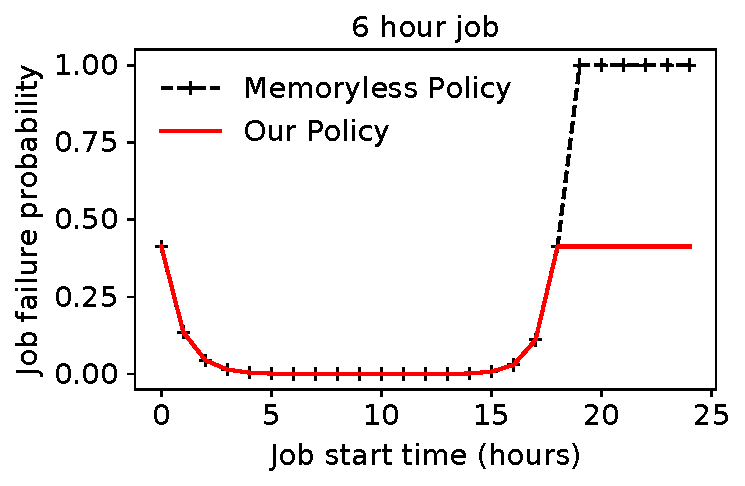
\includegraphics[width=\linewidth]{Sched-bathtub.pdf}
    \vspace*{-0.6cm}
    \caption{Effect of job start time on the failure probability.} \label{fig:sched-bathtub}
  \end{minipage}
  \hfill 
  \begin{minipage}[c]{0.3\linewidth}
    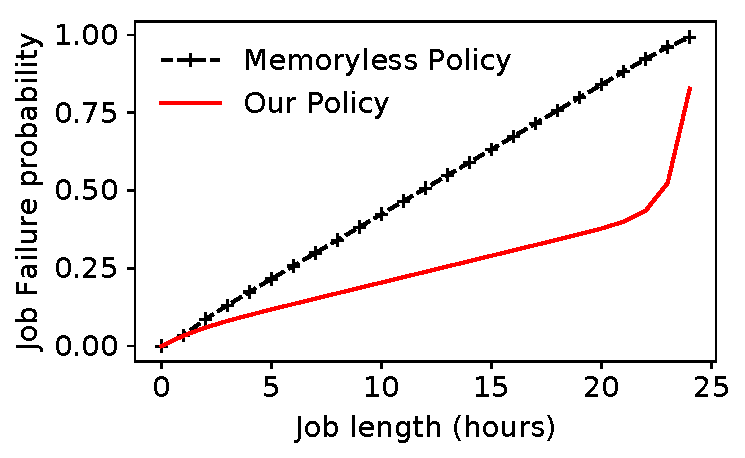
\includegraphics[width=\textwidth]{Sched-fail-prob.pdf}
    \vspace*{-0.6cm}
    \caption{Job failure probability for jobs of different lengths.} \label{fig:sched-all}
  \end{minipage}
  \hfill
  \begin{minipage}[c]{0.3\linewidth}
    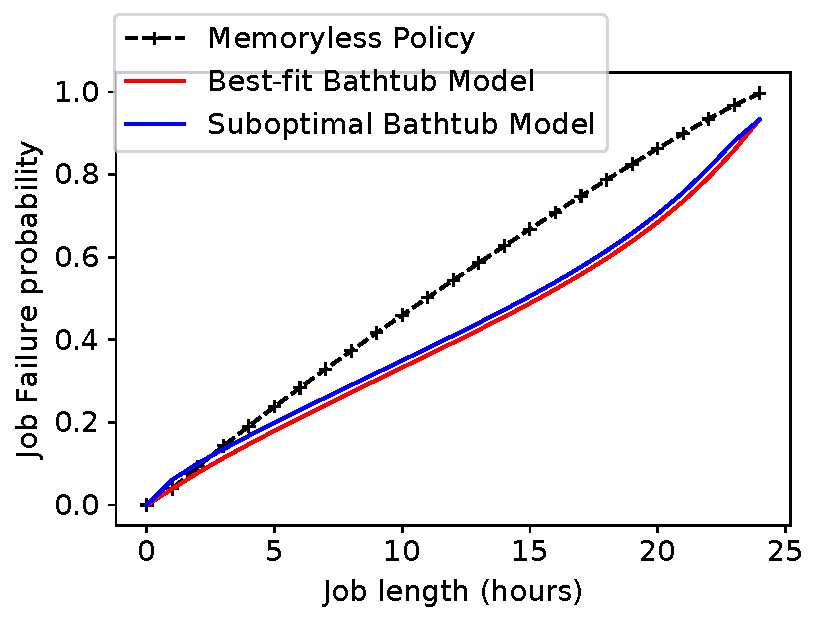
\includegraphics[width=\linewidth]{wrong-model.pdf}
    \vspace*{-0.8cm}
  \caption{Impact of suboptimal bathtub model parameters on the scheduling policy is negligible.}
  \label{fig:wrong-model}
\end{minipage}
\vspace*{-0.4cm}
\end{figure*}


In many scenarios, a server may be used for running a long-running sequence of jobs, such as in a batch-computing service. 
SciSpot's job scheduling policy is model-driven and decides whether to request a new VM for a job or run it on an existing VM.
A new VM may be preferable if the job starts running near the VM's 24 hour preemption deadline.

Figure~\ref{fig:sched-bathtub} shows the effect our job scheduling policy for a six hour job, for different job starting times (relative to the VM's starting time). 
We compare against a baseline of memoryless job scheduling that is not informed by constrained preemption dynamics.
Such memoryless policies are the default in existing transient computing systems such as SpotOn~\cite{spoton}. 
In the absence of insights about bathtub-shaped preemption probability, the memoryless policy continues to run jobs on the existing VM. 
As the figure shows, the empirical job failure probability is bathtub shaped. 
However, because the job is 6 hours long, it will always fail with the memoryless policy when launched after $24-6=18$ hours.
In contrast, \sysname's model-based policy determines that after 18 hours, we will be better off running the job on a newer VM, and results in a constant lower job failure probability ($=0.4$). The failure probability is constant because the jobs will always be launched on a new VM after 18 hours, resulting in a failure probability at time $=0$. 
Thus, \sysname can reduce job failure probability by taking into account the time-varying failure rates of VMs, which is not considered by existing systems that use memoryless scheduling policies. 







The job failure probability is determined by the job length and the job starting time.
We examine the failure probability for jobs of different lengths (uniformly distributed) in Figure~\ref{fig:sched-all}, in which we average the failure probability across different start times.
We again see that our policy results in significantly lower failure probability compared to memoryless scheduling.
For all but the shortest and longest jobs, the failure probability with our policy is \emph{half} of that of existing memoryless policies. 
This reduction is primarily due to how the two policies perform for jobs launched near the end of the VM preemption deadline, which we examined previously in Figure~\ref{fig:sched-bathtub}. 




\noindent \textbf{Sensitivity to model fitting.}
The effectiveness of any model-based policy depends on the goodness of fit of the preemption model---i.e., how accurately it captures empirical data. 
We now evaluate the impact on our scheduling policy if incorrect/suboptimal model parameters with high goodness-of-fit ($r^2$) error are used. 
That is, we seek to understand how sensitive our policies are when the underlying preemption behavior does not match the model, which can occur due to changes in supply/demand, minor cloud policy changes, etc. 
Figure~\ref{fig:wrong-model} compares the job failure probability with the optimal bathtub model that best fits the empirical data, and a suboptimal  bathtub model intentionally chosen to have a bad fit. 
Specifically, the suboptimal case models the \texttt{n1-highcpu-16} VMs for \texttt{n1-highcpu-32} VMs, which from Figure~\ref{fig:cdf-comparison} we can see are significantly different.
However, even with the suboptimal model, the increase in job failure probability is less than 2\% compared to the best-fit model. 
This negligible difference is due to the fact that even a suboptimal model captures the bathtub shape, and this is enough for the policy to make the ``right'' scheduling decision. 

\noindent \textbf{Result:} \emph{\sysname's policies are not particularly sensitive to the exact model parameters, so long as a bathtub distribution is used. Even a suboptimal bathtub model can reduce failure probability by 15\% compared to the memoryless policy.} 


    



\subsection{Impact of VM Selection}


When an application (i.e., bag of jobs) requests a total number of CPUs to run each of its jobs, \sysname first runs its exploration phase to find the ``right'' VM for the application.
\sysname searches for the VM that minimizes the total expected cost $E[C_{(i,n_i)}]$ of running the application. 
Thus, even if the \emph{total} amount of resources (i.e., number of CPUs) per job is held constant, the total running time (i.e., turnaround time) of an application depends on the choice of the VM type ($i$), and the associated number of VMs ($n_i$) required to meet the allocation constraint. 

\begin{figure}
  \centering
  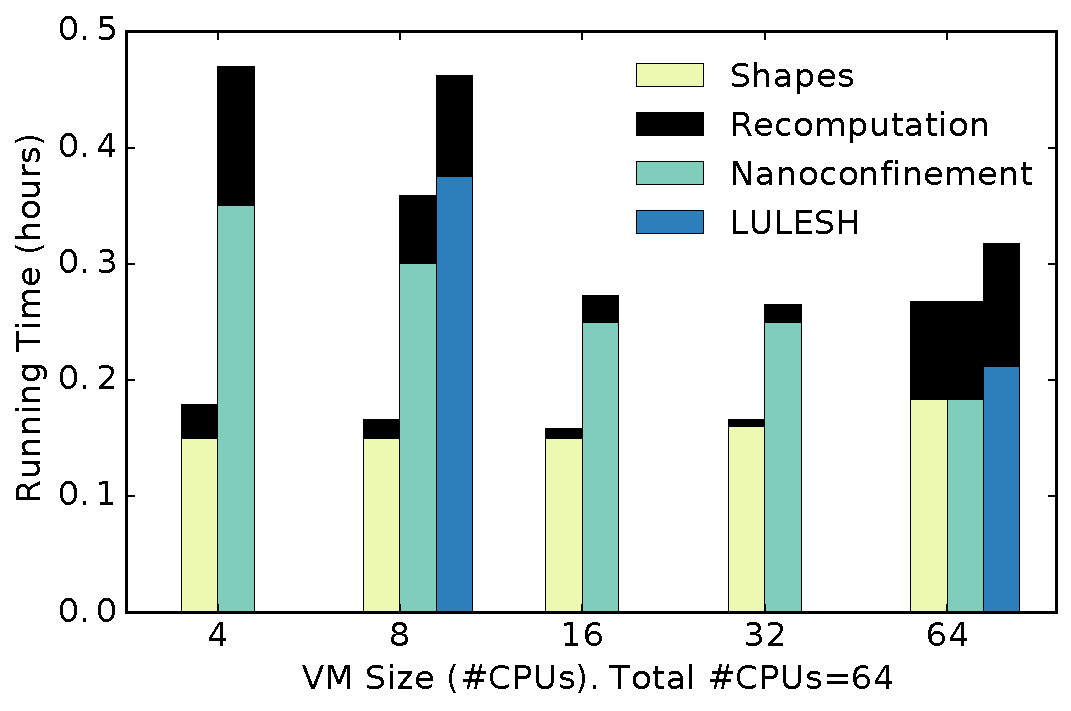
\includegraphics[width=0.4\textwidth]{runtime-bars.pdf}
      \vspace*{\myfigspace}
  \caption{Running times of applications on different VMs. Total number of CPUs is 64, yielding different number of VMs in each case. We see different tradeoffs in the base running times and recomputation times.}
  \label{fig:runtimes-bar}
    \vspace*{\myfigspace}
\end{figure}


Figure~\ref{fig:runtimes-bar} shows the running times of the Nanoconfinement, Shapes, and LULESH applications, when they are deployed on different VM sizes. 
In all cases, the total number of CPUs per job is set to 64, and thus the different VM sizes yield different cluster sizes (e.g., 16 VMs with 4 CPUs or 32 VMs with 2 CPUs).
This experiment does not measure scaling behavior, but instead highlights the differences between choices of VMs. 
LULESH requires CPUs to be cube of an integer, which limits the valid cluster configurations.


For Nanoconfinement and LULESH, we observe that the base running times (without preemptions) reduce when moving to larger VMs, because this entails lower communication costs.
For Nanoconfinement, the running time on the ``best'' VM (i.e., with 32 CPUs) is nearly 40\% lower as compared to the worst case. 
On the other hand, the Shapes application can scale to a larger number of VMs, because the application  does not have any significant communication overheads, and thus does not see any significant change in its running time when deployed on different kind of VMs. 

Figure~\ref{fig:runtimes-bar} also shows the expected recomputation time which depends on the expected lifetimes of the VM and the number of VMs. 
This recomputation time is roughly proportional to the original running time, in accordance with Equation~\ref{eq:wasted}. 
While selecting larger VMs may reduce communication overheads and thus improve performance, it is not an adequate policy in the case of preemptible VMs, since the preemptions can significantly increase the turnaround time.
Therefore, even though the base running time of Nanoconfinement is lower on a 64 CPU VM, the recomputation time on the 64 CPU VM is almost $4\times$ higher compared to a 2x32-CPU cluster,  due to the much lower expected lifetime of the larger VMs. 
Thus, on preemptible servers, there is a tradeoff between the base running time which only considers parallelization overheads, and the recomputation time.
By considering \emph{both} these factors, \sysname's server selection policy can select the best VM for an application. 


\noindent \textbf{Result:} \emph{SciSpot's server selection, by considering both the base running time and recomputation time, can improve performance by up to 40\%, and can keep the increase in running time due to preemptions to less than 5\%.}

\subsection{Cost}

\begin{figure}
  \centering
  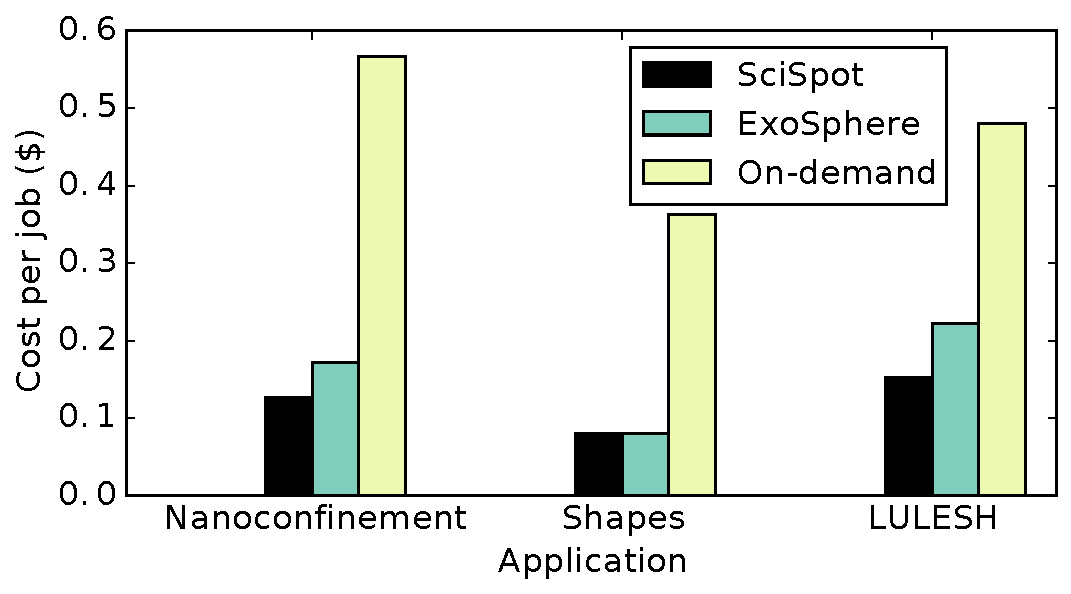
\includegraphics[width=0.4\textwidth]{cost-vs-exosphere.pdf}
  \vspace*{\myfigspace}
  \caption{SciSpot's use of preemptible VMs can reduce costs by up to $5\times$ compared to conventional cloud deployments, and 20\% compared to the state of the art EC2 spot instance selection (ExoSphere~\cite{exosphere}).}
  \label{fig:cost-only-bar}
    \vspace*{\myfigspace}
\end{figure}

The primary motivation for using preemptible VMs is their significantly lower cost compared to conventional ``on-demand'' cloud VMs that are non-preemptible. 
Figure~\ref{fig:cost-only-bar} compares the cost of running different applications with different cloud VM deployments. 
\sysname, which uses both cost-minimizing server selection, and preemptible VMs, results in significantly lower costs across the board, even when accounting for preemptions and recomputations. 
We also compare against ExoSphere~\cite{exosphere}, a state of the art  system for transient server selection.
ExoSphere implements a portfolio-theory approach using EC2 spot prices to balance average cost saving and risk of revocations using diversification and selecting VMs with low price correlation.
However, this approach is ineffective for the flat prices of Google Preemptible VMs. 
Unlike \sysname, ExoSphere does \emph{not} consider application performance when selecting servers, and thus is unable to select the best server for parallel applications. 
Since the Google \texttt{highcpu} VMs have the same price per CPU, ExoSphere picks an arbitrary ``median'' VM to break ties, which may not necessarily yield the lowest running times.
This results in 20\% cost increase over \sysname. 

\noindent \textbf{Result:} \emph{SciSpot reduces computing costs by up to 5$\times$ compared to conventional on-demand cloud deployments.}


\subsection{Comparison with HPC Overhead}

Scientific computing applications are typically run on large-scale HPC clusters, where different performance and cost dynamics apply. 
While there are hardware differences between cloud VMs and HPC clusters that can contribute to performance differences, we are interested in the performance ``overheads''.
In the case of \sysname, the job failures and recomputations increase the job turnaround time, and are thus the main source of overhead. 

On HPC clusters, jobs enjoy significantly lower recomputation probability, since the hardware on these clusters has MTTFs in the range of years to centuries~\cite{dongarra_fault_nodate}.
However, we emphasize that there exist \emph{other} sources of performance overheads in HPC clusters.
In particular, since HPC clusters have high resource utilization, they also have significant \emph{waiting} times. 
On the other hand, cloud resource utilization is low~\cite{borg} and there is usually no need to wait for resources, which is why transient servers exist in the first place. 


Thus, we compare the performance overhead due to preemptions for \sysname, and job waiting times in conventional HPC deployments.
To obtain the job waiting times in HPC clusters, we use the LANL Mustang traces published as part of the Atlas trace repository~\cite{cmu-atlas}. 
We analyze the waiting time of over two million jobs submitted over a 5 year period, and compute the increase in running time of the job due to the job waiting or queuing time. 

\begin{figure}[t]
  \centering 
  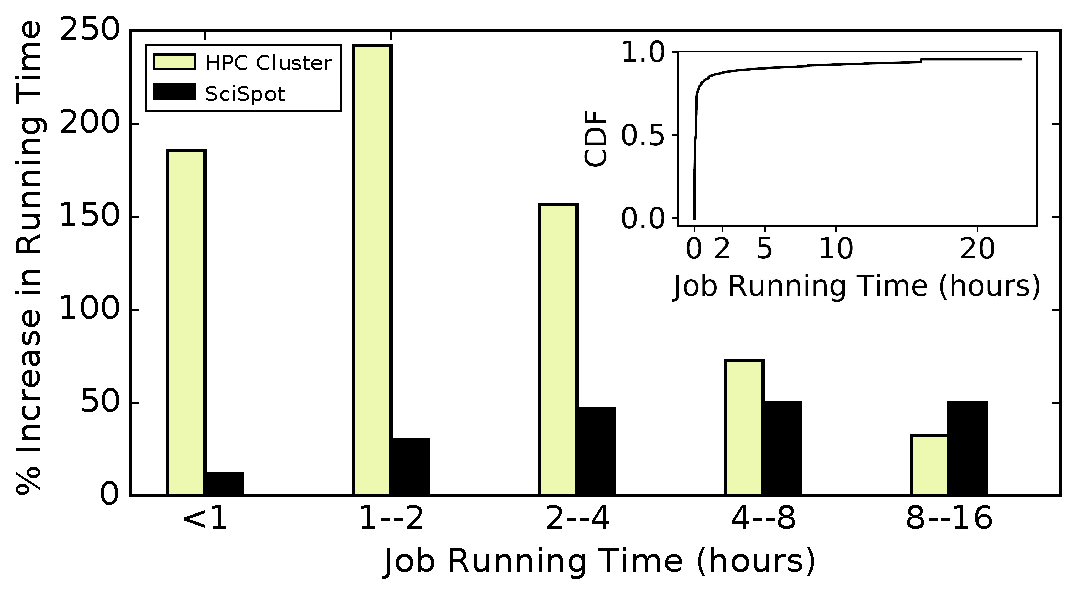
\includegraphics[width=0.4\textwidth]{hpc-vs-scispot.pdf}
      \vspace*{\myfigspace}
  \caption{Increase in running time due to waiting on HPC clusters is significantly higher than the recomputation time for \sysname, except for very long and rare jobs (see inset). }
  \label{fig:hpc-vs-scispot}
  \vspace*{\myfigspace}
\end{figure}


Figure~\ref{fig:hpc-vs-scispot} compares the overhead (as percentage increase in running time) of \sysname and HPC clusters  for jobs of different lengths. We see that the average performance overhead due to waiting can be significant in the case of HPC clusters, and the job submission latency and queuing time dominate for smaller jobs, increasing their total turnaround time by more than $2.5\times$.
This waiting is amortized in the case of longer running jobs, and the overhead for longer jobs is around 30\%.

On the other hand, \sysname's performance overhead is significantly smaller for jobs of up to 8 hours in length.
For longer jobs, the limited lifetime of Google Preemptible VMs (24 hours) begins to significantly increase the preemption probability and expected recomputation time.
We emphasize that these are \emph{individual} job lengths, and not the running time of entire bag of jobs.
We note that these large single jobs are rare, accounting for less than 5\% of all HPC jobs (see inset in Figure~\ref{fig:hpc-vs-scispot}).
For smaller jobs (within a much larger bag), both the preemption probability and recomputation overhead is much smaller.

\noindent \textbf{Result:} \emph{\sysname's overhead of recomputation due to preemptions is small, and is up to $10\times$ lower compared to the overhead of waiting in conventional HPC clusters. }

We emphasize that our goal is to compare the expected waiting time in HPC clusters vs. SciSpot's preemption overheads.
The exact waiting time and performance is dependent on the specific HPC scheduler and hardware: we merely want to highlight that the performance overhead of preemptible VMs is reasonable if users do not wish to wait for HPC resources. 










 

\vspace*{\subsecspace}
\section{Discussion}
\label{sec:discussion}


Constrained preemptions are a relatively unexplored phenomenon and challenging to model.
Our model and the associated data expand transient cloud computing to beyond EC2-spot.
However, many questions and avenues of future investigation remain open:

\noindent \textbf{What if preemption characteristics change?}
Our model allows detecting policy and phase changes by comparing observed data with model-predictions and detect change-points, and 
a long-running cloud service can continuously update the model based on recent preemption behavior. 
However, changes are rare: Google's preemption policy has not changed since its inception in 2015. 
We have also shown that our policies are not particularly sensitive to the model parameters, and even using a poorly-fitted or outdated model can provide significant benefits compared to existing memoryless models. 
Our modeling approach works across a wide range of instance types and is able to model CDFs of instances with both very high and very low failure rates, and thus is general. Moreover, because bathtub preemptions are good for the applications, they will continue to remain a good choice for constrained preemptions making our approach generalizable to other system environments beyond the Google cloud computing systems. Finally, the principle adopted to break down the problem into the superposition of processes characterized by different failure rates can also be considered as a general framework to understand and guide policies for mitigating preemption-induced effects in other cloud environments.

For robust long-term relevance of the preemption model, we envision a community-driven approach.
An increase in SciSpot use by the research community will provide more preemption data, which can then be used to constantly refine the model when preemption characteristics change due to cloud policies or supply/demand fluctuations. 

\noindent \textbf{Generalizability to other Transient VMs.}
In this paper, we focus on constrained preemptions.
Other cloud transient VMs such as spot instances do not have the temporal constraint, and their preemption modeling can be performed with classical distributions (such as exponential distribution for modeling EC2 spot instance preemptions ~\cite{bid-cloud, flint, hotcloud-not-bid}). 
However, we have shown that an empirical approach of collecting actual preemption data is feasible and effective, and a principled approach can be used even without spot-market price signals. 







 

 \section{Conclusion}
 \label{sec:conclusion}


 The effective use of transient computing relies on understanding the preemption characteristics.
While past work on transient computing has developed techniques and systems for Amazon's EC2 spot instances, ours is the \emph{first} work to understand the behavior of Google's Preemptible VMs, that have a unique characteristic of having a maximum 24 hour lifetime.
Our large-scale empirical study shows that the constraint imposes a bathtub failure distribution, and we develop a new preemption probability model for capturing its three distinct temporal phases. 
Our insights and model-based policies can reduce the preemption overheads by more than $5\times$ compared to existing preemption models, and our batch computing service can reduce computing costs by over $5\times$. 


\noindent \textbf{Acknowledgments.}
This research was supported by Google cloud credits for research. 
J.K. and V.J. were partially supported by Department of Energy through Award DE-SC0021418. P.S. was partially supported by NSF OAC-2112606. 


{
\bibliographystyle{abbrv}
\interlinepenalty=10000 
\bibliography{scicloud,bagsjobs,spot-bid}
}



\begin{IEEEbiography}[{
\includegraphics[width=1in,height=1.25in,clip,keepaspectratio]{Kadupitiya_JCS.jpg}}]
{JCS Kadupitiya} is a Ph.D. candidate in the Department of Intelligent Systems Engineering at Indiana University Bloomington. He received a Master's in Computer Engineering from Indiana University Bloomington in 2019.  His research interests lie primarily in scientific machine learning and distributed computing. He completed his Bachelor’s degree in Electrical and Information Engineering from the University of Ruhuna, Sri Lanka, in 2015. He also received a Master's in Computer Science and Engineering at the University of Moratuwa, Sri Lanka, in 2017.
\end{IEEEbiography}


\begin{IEEEbiography}[{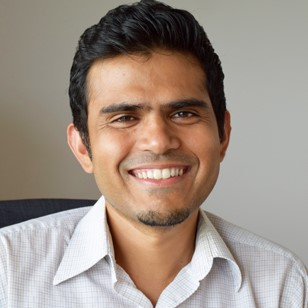
\includegraphics[width=1in,height=1.25in,clip,keepaspectratio]{jadhao-vikram-2016-08.jpg}}]
 {Vikram Jadhao} is an assistant professor of Intelligent Systems Engineering at Indiana University in Bloomington. Prior to joining Indiana University, he held postdoctoral fellowships in the Department of Physics and Astronomy at Johns Hopkins University as well as the Department of Materials Science and Engineering at Northwestern University. He received his Ph.D. and M.S. in Physics from the University of Illinois at Urbana-Champaign, and his B.S. in Physics from the Indian Institute of Technology at Kharagpur. His research interests are broadly in computational modeling and simulation of soft materials at the nanoscale. 
\end{IEEEbiography}



\begin{IEEEbiography}[{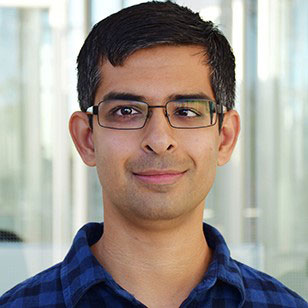
\includegraphics[width=1in,height=1.25in,clip,keepaspectratio]{prateeks.jpg}}]{Prateek Sharma}
  is an an assistant professor of Intelligent Systems Engineering at Indiana University in Bloomington. He has a PhD in Computer Science from 
the University of Massachusetts Amherst. His current research
  focuses on Cloud Computing, Operating Systems, and
  Virtualization. Sharma received his masters degree in Computer Science from
  Indian Institute of Technology, Bombay. Contact him at
  prateeks@iu.edu.
\end{IEEEbiography}




 
\end{document}
